\chapter{El hidrógeno y el bloque s}\label{ch:b1:s-block}

Todo teléfono, todo portátil y todo coche eléctrico lleva una batería
cuyas cargas positivas transportan iones litio. Ese litio procede sobre
todo de dos lugares: las minas de roca dura de Australia y los salares de
los Andes, donde una salmuera bombeada desde debajo de la costra se deja
evaporar al sol durante meses, hasta que pueden precipitarse de ella las
sales de litio. El litio es el primero de los \omterm{def:b1:s-block:families}{metales alcalinos}, los
metales más reactivos que existen, y sus vecinos sodio, potasio, magnesio
y calcio suministran los productos químicos básicos de la industria: la
sosa cáustica, el carbonato de sodio, la cal. Este capítulo abre la
química descriptiva de los elementos con el hidrógeno y el \omterm{def:b1:periodicity:table}{bloque} s, y
usa las herramientas de los capítulos anteriores --- energías de
ionización, \omterm{def:b1:nernst:electrode-potential}{potenciales estándar}, \omterm{def:b1:precipitation:solubility-product}{productos de solubilidad} --- para
explicar lo que hacen estos elementos.

\begin{recall}
Las energías de ionización y la \omterm{def:b1:periodicity:electronegativity}{electronegatividad}
(\cref{ch:b1:periodicity}); los \omterm{def:b1:nernst:electrode-potential}{potenciales estándar}
(\cref{ch:b1:nernst}); los \omterm{def:b1:precipitation:solubility-product}{productos de solubilidad} y la precipitación de
los hidróxidos (\cref{ch:b1:precipitation}). El volumen escolar (año 10)
agrupó los elementos en familias: \omterm{def:b1:s-block:families}{metales alcalinos}, \omterm{def:b1:s-block:families}{metales
alcalinotérreos}, halógenos, gases nobles.
\end{recall}

\begin{omfigure}
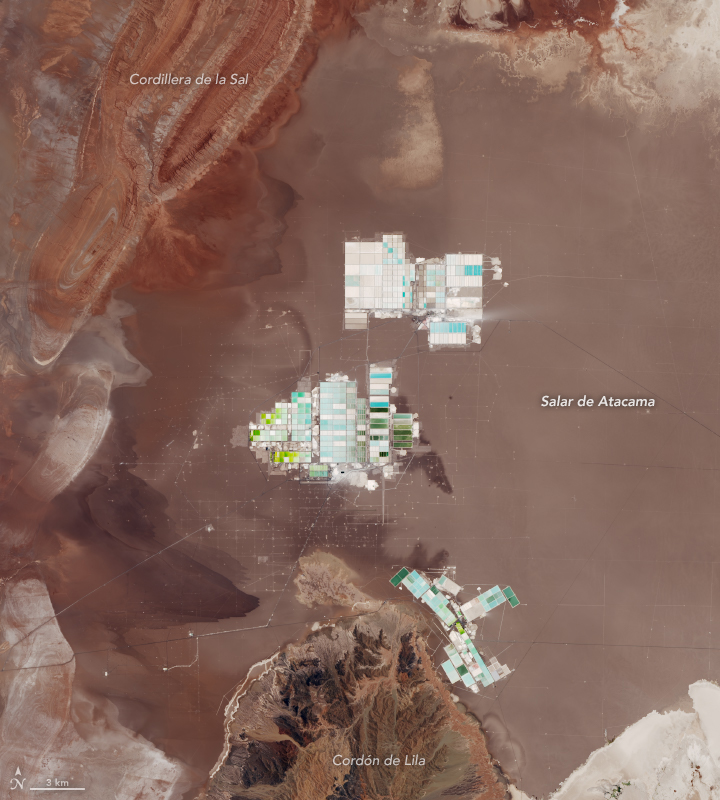
\includegraphics[width=0.48\linewidth]{images/book2/atacama-ponds.jpg}

{\small Piscinas de evaporación de salmuera de litio en el Salar de
Atacama, vistas desde la órbita (Landsat 8, 2018; NASA Earth Observatory,
dominio público, Wikimedia Commons). El color de cada piscina cambia a
medida que la salmuera se concentra y las sales cristalizan.}
\end{omfigure}

\section{El hidrógeno y los hidruros}

El hidrógeno tiene un electrón: puede perderlo (\ce{H+}, que el agua
transporta como \ce{H3O+}), compartirlo (\omterm{def:b1:lewis-resonance-vsepr:lewis}{enlaces covalentes}) o ganar uno
(\ce{H-}, con la \omterm{def:b1:quantum-numbers:configuration}{configuración electrónica} del helio). Lo que haga depende
de su compañero.

\begin{definition}[Hidruros]\label{def:b1:s-block:hydride}
Un \emph{hidruro}\index{hidruro} es un compuesto binario del hidrógeno con
otro elemento. Los \emph{hidruros salinos}\index{hidruro salino}, que
forma con los \omterm{def:b1:s-block:families}{metales alcalinos} y los alcalinotérreos más pesados
(\ce{LiH}, \ce{NaH}, \ce{CaH2}), son sólidos iónicos que contienen
\ce{H-}. Los \emph{hidruros covalentes}\index{hidruro covalente}, que
forma con los elementos del \omterm{def:b1:periodicity:table}{bloque} p (\ce{CH4}, \ce{NH3}, \ce{H2O},
\ce{HCl}), son moleculares. Los \emph{hidruros metálicos}\index{hidruro metalico@hidruro metálico}, que
forma con algunos metales de transición, son sólidos en los que el
hidrógeno ocupa \omterm{def:b1:crystals-metals:site}{huecos intersticiales} de la \omterm{def:b1:crystals-metals:lattice}{red} del metal, a menudo con
una composición variable.
\end{definition}

El ion \omterm{def:b1:s-block:hydride}{hidruro} es una base y un \omterm{def:b1:nernst:couple}{reductor} muy fuertes: los \omterm{def:b1:s-block:hydride}{hidruros
salinos} reaccionan con el agua, \ce{NaH + H2O -> NaOH + H2}, y sirven
como agentes desecantes de disolventes y como bases en síntesis orgánica
(\cref{ch:b1:alcohol-activation}). Los \omterm{def:b1:s-block:hydride}{hidruros covalentes} del segundo
\omterm{def:b1:periodicity:table}{periodo} muestran la tendencia de la \omterm{def:b1:periodicity:electronegativity}{electronegatividad} a lo largo de él:
\ce{CH4}, ni ácido ni básico; \ce{NH3}, básico; \ce{H2O}, anfótero;
\ce{HF}, ácido.

\section{Los metales alcalinos}

\begin{definition}[Metales alcalinos y alcalinotérreos]\label{def:b1:s-block:families}
Los \emph{metales alcalinos}\index{metal alcalino} (Li, Na, K, Rb, Cs, Fr)
forman el \omterm{def:b1:periodicity:table}{grupo} 1, con un electrón de valencia \textit{ns}$^1$; los
\emph{metales alcalinotérreos}\index{metal alcalinoterreo@metal alcalinotérreo} (Be, Mg, Ca, Sr,
Ba, Ra) forman el \omterm{def:b1:periodicity:table}{grupo} 2, con \textit{ns}$^2$. Sus elementos constituyen
el \omterm{def:b1:periodicity:table}{bloque} s.
\end{definition}

\begin{proposition}[Los metales alcalinos son reductores fuertes]\label{prop:b1:s-block:reducing-power}
Los \omterm{def:b1:s-block:families}{metales alcalinos} tienen las \omterm{def:b1:periodicity:ionisation-energy}{primeras energías de ionización} más
bajas de sus \omterm{def:b1:periodicity:table}{periodos} (Li \qty{5.39}{eV}, Na 5.14, K 4.34) y \omterm{def:b1:nernst:electrode-potential}{potenciales
estándar} muy negativos (\ce{Li+}/\ce{Li} $-3.04$~V, \ce{Na+}/\ce{Na}
$-2.71$, \ce{K+}/\ce{K} $-2.94$): reducen el agua y en la naturaleza solo
se encuentran como iones \ce{M+}.
\end{proposition}
% ledger: ie:Li, ie:Na, ie:K (E0 computed in figdata/bachelor-1/standard-potentials.py)

\begin{proof}
Un único electrón fuera de un núcleo de gas noble, lejos del núcleo y
apantallado por las capas internas (\cref{ch:b1:periodicity}), se
arranca con facilidad. En agua, el pequeño ion \ce{M+} está fuertemente
hidratado, lo que hace aún más bajo el potencial del par. Con un
$E^\circ$ más de \qty{2.2}{V} por debajo de la recta del agua a pH 7
($-0.41$~V), la reacción \ce{2M + 2H2O -> 2M+ + 2OH- + H2} tiene una
constante enorme
(\cref{prop:b1:nernst:equilibrium-constant}).
\end{proof}

\begin{omfigure}
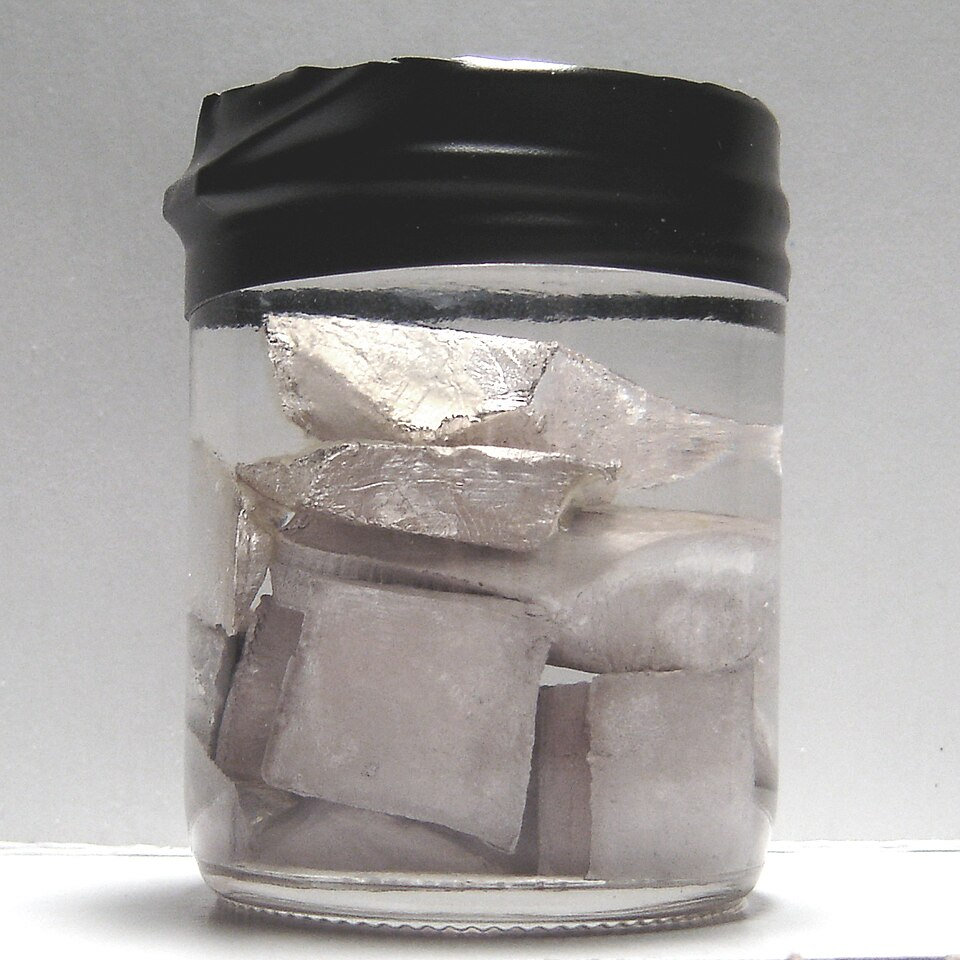
\includegraphics[height=4.6cm]{images/book2/sodium-oil.jpg}\hspace{0.8em}%
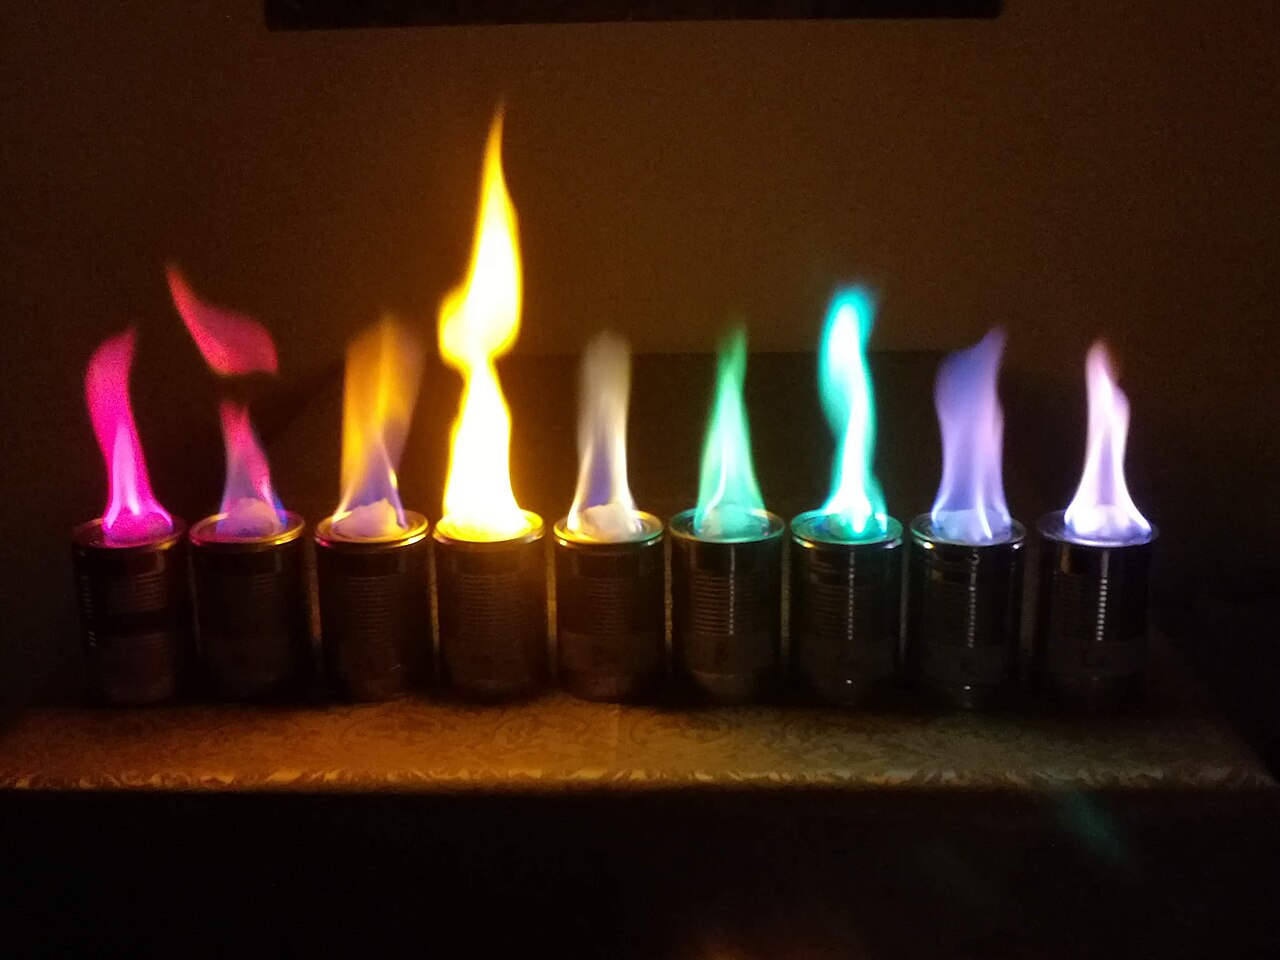
\includegraphics[height=4.6cm]{images/book2/flame-colours.jpg}

{\small Izquierda: el sodio se guarda bajo aceite mineral, lejos del aire
y de la humedad (fotografía de Justin Urgitis, CC BY-SA 2.5). Derecha:
colores de llama, de izquierda a derecha, de compuestos de litio,
estroncio, calcio, sodio, bario, boro, cobre, cesio y potasio: los
electrones excitados en la llama vuelven a niveles más bajos emitiendo
luz de longitudes de onda características de cada elemento
(\cref{ch:b1:quantum-numbers}) (fotografía de Hegelrast, CC BY-SA 4.0).
Ambas de Wikimedia Commons.}
\end{omfigure}

\begin{inthelab}[Una demostración, no un experimento]
La reacción del sodio con el agua solo la muestra un profesor, detrás de
una pantalla de seguridad, dejando caer un trozo del tamaño de una lenteja
en una gran cubeta de agua con fenolftaleína: el metal se funde en una
bola que corre por la superficie, el hidrógeno burbujea, y la estela rosa
muestra el hidróxido formado. El potasio inflama el hidrógeno. Los trozos
más grandes explotan. El sodio se corta bajo aceite, se manipula con
pinzas, y sus restos se destruyen con etanol, nunca con agua.
\end{inthelab}

El litio es la excepción de su grupo: el ion más pequeño, el más
fuertemente hidratado y, por tanto, el de potencial más negativo, y sin
embargo el más lento en reaccionar con el agua. Sus compuestos se parecen
a los del magnesio (el carbonato y el fosfato de litio son poco solubles,
como los del magnesio): una relación diagonal en la tabla periódica. Los
\omterm{def:b1:s-block:families}{metales alcalinos} se obtienen por electrólisis de sus cloruros fundidos,
pues ningún \omterm{def:b1:nernst:couple}{reductor} químico es lo bastante fuerte; las reacciones de
electrodo de esas celdas se estudian en el volumen del segundo año.

\section{Los compuestos del sodio en la industria}

\begin{definition}[Carácter de los óxidos]\label{def:b1:s-block:oxide-character}
Un \emph{óxido básico}\index{oxido basico@óxido básico} reacciona con el agua para dar un
hidróxido, o con los ácidos para dar sales (\ce{Na2O}, \ce{CaO}); un
\emph{óxido ácido}\index{oxido acido@óxido ácido} reacciona con el agua para dar un ácido, o
con las bases para dar sales (\ce{CO2}, \ce{SO3}, \ce{P4O10}); un
\emph{óxido anfótero}\index{oxido anfotero@óxido anfótero} reacciona a la vez con los ácidos y
con las bases (\ce{Al2O3}, \ce{ZnO}). A lo largo de un \omterm{def:b1:periodicity:table}{periodo}, los
óxidos pasan de básicos (metales, a la izquierda) a ácidos (no metales, a
la derecha).
\end{definition}

El hidróxido de sodio se fabrica por electrólisis de la salmuera (el
proceso cloro-álcali, que también da cloro e hidrógeno). El carbonato de
sodio, la sosa Solvay, que se usa para el vidrio, los detergentes y la
extracción del litio, se extrae como el mineral trona o se fabrica a
partir de sal y de caliza: en 2025 el mundo produjo unos 71 millones de
toneladas, 19 millones de yacimientos naturales y 52 millones de síntesis,
la mayor parte por el proceso Solvay.
% ledger: usgs:sodaash-total-2025, usgs:sodaash-natural-2025, usgs:sodaash-synthetic-2025

\begin{proposition}[El proceso Solvay]\label{prop:b1:s-block:solvay}
El proceso Solvay convierte el cloruro de sodio y el carbonato de calcio
en carbonato de sodio y cloruro de calcio, \ce{2NaCl + CaCO3 -> Na2CO3 +
CaCl2}, mediante etapas en las que se reciclan el amoniaco y el dióxido
de carbono.
\end{proposition}

\begin{proof}
Las etapas son: (1) \ce{CaCO3 -> CaO + CO2} (horno); (2) \ce{NaCl + NH3 +
CO2 + H2O -> NaHCO3 + NH4Cl} (carbonatación de la salmuera amoniacal; el
hidrogenocarbonato, la sal menos soluble presente, precipita); (3)
\ce{2NaHCO3 -> Na2CO3 + CO2 + H2O} (calcinación); (4) \ce{CaO + H2O ->
Ca(OH)2}; (5) \ce{Ca(OH)2 + 2NH4Cl -> CaCl2 + 2NH3 + 2H2O} (recuperación
del amoniaco). Al sumar $(1) + 2\times(2) + (3) + (4) + (5)$, se cancelan
\ce{NH3}, \ce{CO2}, \ce{NH4Cl}, \ce{NaHCO3}, \ce{CaO}, \ce{Ca(OH)2} y el
agua:
\ce{2NaCl + CaCO3 -> Na2CO3 + CaCl2}.
\end{proof}

\begin{omfigure}
\begin{tikzpicture}[font=\small, >={Stealth}, box/.style={draw, rounded corners, fill=omDef!8, minimum width=2.6cm, minimum height=0.8cm, align=center}]
  \node[box] (kiln) at (0,0) {horno de cal\\\ce{CaCO3 -> CaO + CO2}};
  \node[box] (tower) at (5.3,0) {carbonatación\\precipita el \ce{NaHCO3}};
  \node[box] (calc) at (10.2,0) {calcinador\\\ce{NaHCO3} $\to$ \ce{Na2CO3}};
  \node[box] (slake) at (0,-2.6) {apagado de la cal\\\ce{CaO + H2O -> Ca(OH)2}};
  \node[box] (still) at (5.3,-2.6) {destilador\\\ce{NH4Cl + Ca(OH)2}};
  \draw[->, thick] (kiln) -- node[above] {\ce{CO2}} (tower);
  \draw[->, thick] (tower) -- node[above, font=\scriptsize] {\ce{NaHCO3}} (calc);
  \draw[->, thick] (calc.north) -- ++(0,0.6) -| node[pos=0.25, above] {\ce{CO2} reciclado} (tower.north);
  \draw[->, thick] (kiln) -- node[left] {\ce{CaO}} (slake);
  \draw[->, thick] (slake) -- node[above, font=\scriptsize] {\ce{Ca(OH)2}} (still);
  \draw[->, thick] (tower) -- node[right] {\ce{NH4Cl}} (still);
  \draw[->, thick] (still.east) -- ++(1.2,0) |- node[pos=0.25, right] {\ce{NH3} reciclado} ($(tower.east)+(0,-0.25)$);
  \draw[<-, thick] (tower.north west) -- ++(-0.5,0.6) node[above] {salmuera \ce{NaCl}};
  \draw[->, thick] (calc.east) -- ++(0.8,0) node[right] {\ce{Na2CO3}};
  \draw[->, thick] (still.south) -- ++(0,-0.6) node[below] {\ce{CaCl2}};
\end{tikzpicture}

{\small El proceso Solvay. El dióxido de carbono y el amoniaco circulan en
bucles; entran la sal y la caliza, y salen el carbonato de sodio y el
cloruro de calcio.}
\end{omfigure}

\begin{omfigure}
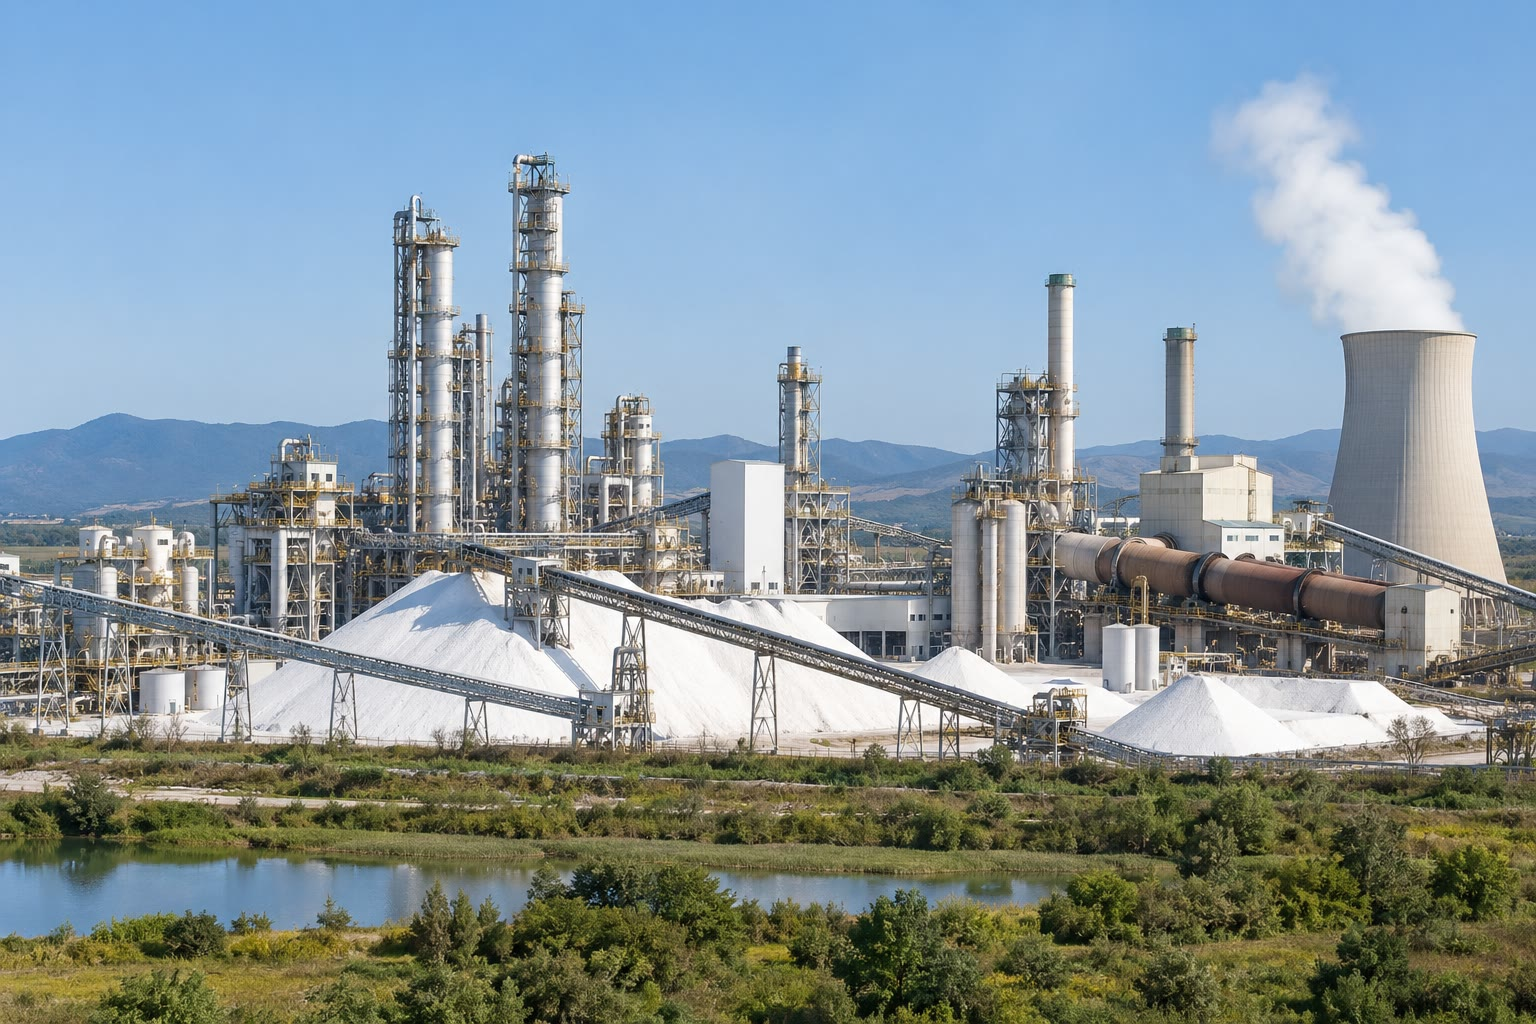
\includegraphics[width=0.55\linewidth]{images/book2/ai/b1-26-soda-ash-plant.jpg}

{\small Una planta de carbonato de sodio: hornos de cal, torres de
carbonatación y acopios de carbonato de sodio.}
\end{omfigure}

\begin{method}[Balance de materia en un diagrama de flujo]\label{met:b1:s-block:mass-balance}
\begin{enumerate}
  \item Se escribe la ecuación global (suma de las etapas, con las
        especies recicladas canceladas).
  \item A partir del producto deseado, se calculan las cantidades de
        materias primas con la ecuación global y después se corrigen con
        el \omterm{def:b1:extent-q-and-k:fractional-extent}{rendimiento} de cada etapa.
  \item Para una especie reciclada, se calcula solo la reposición
        necesaria para compensar sus pérdidas.
  \item Se comprueba el balance de cada elemento entre entradas y salidas.
\end{enumerate}
\end{method}

\section{Los metales alcalinotérreos}

El magnesio y el calcio son menos reactivos que los \omterm{def:b1:s-block:families}{metales alcalinos}
(energías de ionización más altas: Mg \qty{7.65}{eV}, Ca 6.11; dos
electrones que perder), pero siguen siendo \omterm{def:b1:nernst:couple}{reductores} fuertes ($E^\circ$
de \ce{Mg^2+}/\ce{Mg}, $-2.36$~V). El magnesio arde en el aire con una
luz blanca deslumbrante; su película de óxido lo protege a temperatura
ambiente. El magnesio se recupera del agua de mar precipitando su
hidróxido con cal, $\mathrm{p}K_s = 11.25$
(\cref{ch:b1:precipitation}).
% ledger: ie:Mg, ie:Ca

\begin{proposition}[El ciclo de la cal]\label{prop:b1:s-block:lime-cycle}
La caliza, la cal viva, la cal apagada y de nuevo la caliza forman un
ciclo: \ce{CaCO3 -> CaO + CO2} (calentado en un horno);
\ce{CaO + H2O -> Ca(OH)2} (apagado, fuertemente exotérmico);
\ce{Ca(OH)2 + CO2 -> CaCO3 + H2O} (fraguado del mortero de cal al aire).
El ciclo en su conjunto no cambia nada químicamente, pero almacena y
libera energía y dióxido de carbono.
\end{proposition}

\begin{proof}
Al sumar las tres ecuaciones, todas las especies se cancelan. La
descomposición del carbonato requiere calor, que se libera de nuevo en
las otras dos etapas; el \ce{CO2} desprendido en el horno lo vuelve a
captar, lentamente, el mortero.
\end{proof}

\begin{omfigure}
\begin{tikzpicture}[font=\small, >={Stealth}]
  \node[draw, rounded corners, fill=omDef!8] (a) at (90:2.0) {\ce{CaCO3} caliza};
  \node[draw, rounded corners, fill=omDef!8] (b) at (-30:2.0) {\ce{CaO} cal viva};
  \node[draw, rounded corners, fill=omDef!8] (c) at (210:2.0) {\ce{Ca(OH)2} cal apagada};
  \draw[->, thick] (a) to[bend left=25] node[right, align=left] {calor\\$-\ce{CO2}$} (b);
  \draw[->, thick] (b) to[bend left=25] node[below] {$+\ce{H2O}$} (c);
  \draw[->, thick] (c) to[bend left=25] node[left, align=right] {$+\ce{CO2}$\\$-\ce{H2O}$} (a);
\end{tikzpicture}

{\small El ciclo de la cal, de la caliza al mortero y de vuelta al
carbonato de calcio.}
\end{omfigure}

\section{El litio}

\begin{omfigure}
\begin{tikzpicture}
\begin{axis}[
  xbar, width=0.78\linewidth, height=5.4cm, xmin=0, xmax=110,
  symbolic y coords={CA,ML,BR,AR,ZW,CL,CN,AU}, ytick=data,
  yticklabels={Canadá, Malí, Brasil, Argentina, Zimbabue, Chile, China, Australia},
  xlabel={litio extraído en 2025 (miles de toneladas de Li, estimaciones)}, bar width=8pt,
  nodes near coords, every node near coord/.append style={font=\scriptsize},
  tick label style={font=\small}, label style={font=\small}, enlarge y limits=0.1]
\addplot[fill=omDef!45, draw=omDef] coordinates {(5.6,CA) (9.4,ML) (12,BR) (23,AR) (28,ZW) (56,CL) (62,CN) (92,AU)};
\end{axis}
\end{tikzpicture}

{\small Los mayores productores de litio en 2025 (estimaciones; total
mundial, unas \num{290000} toneladas de litio). Australia extrae roca dura
(espodumena); Chile y Argentina bombean salmueras.}
% ledger: usgs:li-canada-2025, usgs:li-mali-2025, usgs:li-brazil-2025, usgs:li-argentina-2025, usgs:li-zimbabwe-2025, usgs:li-chile-2025, usgs:li-china-2025, usgs:li-australia-2025, usgs:li-world-2025
\end{omfigure}

La salmuera se concentra por evaporación, el magnesio se elimina con cal,
y el carbonato de litio se precipita con carbonato de sodio. El carbonato
de litio tiene la propiedad poco habitual de ser menos soluble en
caliente que en frío: \qty{1.31}{\percent} en masa a \qty{20}{\celsius},
\qty{0.84}{\percent} a \qty{80}{\celsius}, \qty{0.71}{\percent} a
\qty{100}{\celsius}. Por eso se precipita en disolución caliente, como
calcula el problema de fin de semana.
% ledger: sol:Li2CO3-20, sol:Li2CO3-80, sol:Li2CO3-100

\section{Ejercicios}

\begin{exercise}[$\star$]\label{exo:b1:s-block:1}
Clasifíquense como \omterm{def:b1:s-block:hydride}{hidruro salino}, covalente o metálico: \ce{KH},
\ce{SiH4}, \ce{CaH2}, \ce{H2S}, \ce{PdH_{0.6}}. Escríbase la reacción del
\ce{CaH2} con el agua.
\end{exercise}

\begin{exercise}[$\star$]\label{exo:b1:s-block:2}
Escríbanse las reacciones del litio, el sodio y el potasio con el agua, y
la del magnesio con ácido clorhídrico diluido.
\end{exercise}

\begin{exercise}[$\star$]\label{exo:b1:s-block:3}
Clasifíquense como básicos, ácidos o anfóteros: \ce{Na2O}, \ce{MgO},
\ce{Al2O3}, \ce{SiO2}, \ce{SO3}, \ce{ZnO}, \ce{CO2}. Escríbase una
reacción de cada tipo.
\end{exercise}

\begin{exercise}[$\star$]\label{exo:b1:s-block:4}
Calcúlese la constante de \ce{2Na + 2H2O -> 2Na+ + 2OH- + H2} a pH 14 a
partir de los \omterm{def:b1:nernst:electrode-potential}{potenciales estándar}.
\end{exercise}

\begin{exercise}[$\star\star$]\label{exo:b1:s-block:5}
Explíquense los colores de llama del litio (rojo) y del sodio (amarillo)
mediante los \omterm{def:b1:quantum-numbers:energy-level}{niveles de energía} de los átomos
(\cref{ch:b1:quantum-numbers}). ¿Cuál es la energía de un fotón amarillo
de \qty{589}{nm}?
\end{exercise}

\begin{exercise}[$\star\star$]\label{exo:b1:s-block:6}
Calcúlense la masa de caliza (\ce{CaCO3} pura) y la de cloruro de sodio
necesarias para una tonelada de carbonato de sodio por el proceso Solvay,
con un \omterm{def:b1:extent-q-and-k:fractional-extent}{rendimiento} global del \qty{90}{\percent} respecto del cloruro de
sodio.
\end{exercise}

\begin{exercise}[$\star\star$]\label{exo:b1:s-block:7}
El agua de mar contiene unos \qty{1.3}{g/L} de magnesio (dato del
ejercicio). ¿A qué pH empieza a precipitar el hidróxido de magnesio? ¿Qué
masa de cal apagada precipita el magnesio de \qty{1.0}{m^3}?
\end{exercise}

\begin{exercise}[$\star\star$]\label{exo:b1:s-block:8}
¿Por qué reacciona el litio con el agua más despacio que el potasio,
aunque su \omterm{def:b1:nernst:electrode-potential}{potencial estándar} sea más bajo? Distíngase entre
termodinámica y cinética.
\end{exercise}

\begin{exercise}[$\star\star$]\label{exo:b1:s-block:9}
Calcúlense la masa de cal viva obtenida a partir de una tonelada de
caliza y el volumen de \ce{CO2} liberado, a \qty{25}{\celsius} y
\qty{1}{bar}.
\end{exercise}

\begin{exercise}[$\star\star\star$]\label{exo:b1:s-block:10}
El mundo extrajo unas \num{290000} toneladas de litio en 2025. ¿Qué masa
de carbonato de litio representa? Si la batería de un coche contiene
\qty{8}{kg} de litio (dato del ejercicio), ¿para cuántas baterías
alcanzaría?
\end{exercise}

\begin{exercise}[$\star\star\star$]\label{exo:b1:s-block:11}
Demuéstrese con los datos del capítulo que la \omterm{def:b1:precipitation:solubility}{solubilidad} del carbonato
de litio disminuye con la temperatura, y explíquese por qué precipitarlo
en caliente mejora su recuperación a partir de una salmuera.
\end{exercise}

\begin{exercise}[$\star\star\star$]\label{exo:b1:s-block:12}
En la etapa (2) del proceso Solvay, la disolución contiene \ce{Na+},
\ce{NH4+}, \ce{Cl-} y \ce{HCO3-}. Explíquese por qué precipita el
hidrogenocarbonato de sodio y no el cloruro de amonio, y por qué el
proceso necesita amoniaco y no hidróxido de sodio.
\end{exercise}

\section{Problema: litio a partir de una salmuera}

\begin{problem}[{Problema de fin de semana --- la concentración de una
salmuera de litio, la eliminación del magnesio con cal, la precipitación
del carbonato de litio con carbonato de sodio, y la masa de carbonato de
litio recuperada de un metro cúbico}]
\label{pb:b1:s-block:1}
Una salmuera bombeada desde debajo de un salar contiene \qty{1.5}{g/L} de
litio y \qty{0.60}{g/L} de magnesio (en forma de iones, con mucho cloruro
de sodio). La evaporación en piscinas la concentra cuatro veces. Se trata
después un metro cúbico de la salmuera concentrada: la cal elimina el
magnesio, el carbonato de sodio el calcio, y finalmente el carbonato de
sodio en caliente precipita el carbonato de litio a \qty{80}{\celsius}.
Datos: masas molares (\unit{g/mol}) Li 6.9, Mg 24.3,
\ce{Ca(OH)2} 74.1, \ce{Na2CO3} 106.0, \ce{Li2CO3} 73.8; $\mathrm{p}K_s$
\ce{Mg(OH)2} 11.25, \ce{CaCO3} 8.30; $\mathrm{p}K_e = 14.00$; \omterm{def:b1:precipitation:solubility}{solubilidad}
del \ce{Li2CO3}, \qty{0.84}{\percent} en masa a \qty{80}{\celsius}; se
toma el líquido final como \qty{1.00}{m^3} de densidad \qty{1.0}{kg/L}.

\medskip
\noindent\textbf{Parte I --- La concentración.}
\begin{enumerate}
  \item Calcúlense las concentraciones de litio y de magnesio en la
        salmuera concentrada.
  \item ¿Qué volumen de agua se evapora por metro cúbico de salmuera
        concentrada?
  \item ¿Por qué se usa la evaporación solar y no el calentamiento?
  \item ¿Qué sal cristaliza primero en las piscinas, y por qué?
  \item Calcúlense las cantidades de litio y de magnesio en un metro
        cúbico.
  \item ¿Por qué hay que eliminar el magnesio antes de precipitar el
        litio?
\end{enumerate}

\medskip
\noindent\textbf{Parte II --- La eliminación del magnesio y del calcio.}
\begin{enumerate}[resume]
  \item Escríbase la reacción de los iones magnesio con la cal apagada.
  \item Calcúlese la masa de cal apagada necesaria (estequiométrica).
  \item ¿A qué pH ha precipitado el \qty{99.9}{\percent} del magnesio?
  \item ¿Por qué no precipita el litio como hidróxido?
  \item Escríbase la eliminación del calcio introducido, con carbonato de
        sodio.
  \item Calcúlese la masa de carbonato de sodio necesaria para esa etapa.
\end{enumerate}

\medskip
\noindent\textbf{Parte III --- El carbonato de litio.}
\begin{enumerate}[resume]
  \item Escríbase la precipitación del carbonato de litio.
  \item Calcúlese la masa de carbonato de sodio necesaria para el litio.
  \item Calcúlese la masa teórica de carbonato de litio.
  \item ¿Por qué se hace la precipitación a \qty{80}{\celsius}?
  \item ¿Qué masa de carbonato de litio queda disuelta en el líquido?
  \item ¿Cómo se lava el precipitado sin perder mucho de él?
\end{enumerate}

\medskip
\noindent\textbf{Parte IV --- El balance.}
\begin{enumerate}[resume]
  \item Calcúlese la masa de carbonato de litio recuperada.
  \item Calcúlese el \omterm{def:b1:extent-q-and-k:fractional-extent}{rendimiento} de recuperación del litio.
  \item Sugiérase qué se hace con el líquido.
  \item Compárese el litio de un metro cúbico con la producción mundial de
        2025: ¿cuántos metros cúbicos representaría esa producción?
  \item Dese la masa de carbonato de litio recuperada por metro cúbico de
        salmuera concentrada.
\end{enumerate}
\end{problem}
